% Micha�l Baudin, 2017
\documentclass{article}

% Copyright (C) 2012 - 2013 - EDF R&D - Michael Baudin

\setbeameroption{hide notes}
%\setbeameroption{show notes}
%\setbeameroption{show only notes}
%\mode<presentation>{\usetheme{EDF09}}

% Configuration beamer
\usetheme{Montpellier}
\setbeamertemplate{navigation symbols}{} % Remove navigation
\useoutertheme{infolines}
\setbeamertemplate{theorems}[numbered] 
% Utilise des fonts serif, pour �viter les pb de fonte
\usefonttheme{serif} 
\setbeamertemplate{caption}[numbered]


\usepackage[utf8]{inputenc}
\usepackage[T1]{fontenc}


\usepackage[french]{babel}
\uselanguage{French}
\languagepath{French}

% Scilab macros
\newcommand{\sciobj}[1]{\texttt{#1}}
\newcommand{\scifile}[1]{\texttt{#1}}

% Python macros
\newcommand{\pyobj}[1]{\textcolor{blue}{\texttt{#1}}}

\def\RR{\mathbb{R}}
\def\NN{\mathbb{N}}
\def\ZZ{\mathbb{Z}}
\def\bx{{\bf x}}

% To highlight source code
\usepackage{listingsutf8}
\lstset{inputencoding=utf8/latin1}

\definecolor{darkgreen}{rgb}{0,0.5,0}
\definecolor{violet}{rgb}{0.5,0,1}
\lstset{
  % general command to set parameter(s)
   basicstyle=\scriptsize\ttfamily, %
   keywordstyle=\color{violet}\bfseries,%
   commentstyle=\color{darkgreen}\bfseries,%
   showspaces=false,%
   stringstyle=\color{red}\bfseries
}

\hypersetup{
    %bookmarks=true,         % show bookmarks bar?
    %unicode=false,          % non-Latin characters in Acrobat�s bookmarks
    %pdftoolbar=true,        % show Acrobat�s toolbar?
    %pdfmenubar=true,        % show Acrobat�s menu?
    %pdffitwindow=false,     % window fit to page when opened
    %pdfstartview={FitH},    % fits the width of the page to the window
    %pdftitle={My title},    % title
    %pdfauthor={Author},     % author
    %pdfsubject={Subject},   % subject of the document
    %pdfcreator={Creator},   % creator of the document
    %pdfproducer={Producer}, % producer of the document
    %pdfkeywords={keyword1} {key2} {key3}, % list of keywords
    %pdfnewwindow=true,      % links in new window
    colorlinks=true,       % false: boxed links; true: colored links
    %linkcolor=red,          % color of internal links (change box color with linkbordercolor)
    %citecolor=green,        % color of links to bibliography
    %filecolor=magenta,      % color of file links
    urlcolor=blue           % color of external links
}

%%%%%%%%%%%%%%%%%%%%%%%%%%%%%%%%%%%%%%%%%%%%%%%%%%%%%%%%%%%%%%%%%%%

\begin{document}


\title{OpenTURNS and its graphical interface}

\author{
	Micha�l Baudin$^1$
	\and
Anne Dutfoy$^1$
	\and
Anthony Geay$^1$
	\and
Ovidiu Mircescu$^1$
	\and
Thibault Delage$^1$
	\and
Aur�lie Ladier$^2$
	\and
Julien Schueller$^2$
	\and
Thierry Yalamas$^2$
}


%\author[1]{Micha�l Baudin}
%\author[1]{Anne Dutfoy}
%\author[1]{Anthony Geay}
%\author[1]{Ovidiu Mircescu}
%\author[1]{Thibault Delage}
%\author[2]{Aur�lie Ladier}
%\author[2]{Julien Schueller}
%\author[2]{Thierry Yalamas}
%\affil[1]{Phimeca Engineering. 18/20 boulevard de Reuilly, 75012 Paris - France, yalamas@phimeca.com}
%\affil[2]{EDF R\&D. 6, quai Watier, 78401, Chatou Cedex - France, michael.baudin@edf.fr}

\maketitle

\begin{center}
$^1$ EDF R\&D. 6, quai Watier,
	78401, Chatou Cedex - France,
	michael.baudin@edf.fr

$^2$ Phimeca Engineering.
18/20 boulevard de Reuilly, 
75012 Paris - France,  \\
yalamas@phimeca.com
\end{center}


\abstract{
OpenTURNS is an open source library for uncertainty propagation by 
probabilistic methods. 
Developed in a partnership of four industrial companies (EDF, Airbus, 
Phimeca and IMACS), it benefits from a strong practical feed-back. 
Classical algorithms of UQ are available : central dispersion, 
probability of exceedance, sensitivity analysis, metamodels and 
stochastic processes. 
Developped in C++, OpenTURNS is also available as a Python module and 
has gained maturity thanks to more than 10 years of development. 
However, there are situations where the engineer in charge of 
performing an uncertainty study does not want to use a programming 
language such as C++ or Python. 
% In this context, providing a graphical user interface (GUI) may allow 
% to greatly increase the use of OpenTURNS and, more generally, of the 
% UQ methodology. 

In this talk, we will present a basic tutorial of OpenTURNS in Python 
and will review the new features in the library, which include 
new incremental statistical estimators. 
% Finally, the new features included in the open source GUI will be 
% presented, including the management of stochastic processes. 
}

\tableofcontents

%%%%%%%%%%%%%%%%%%%%%%%%%%%%%%%%%%%%%%%%%%%%%%%%%

\section{Introduction}
The number of software for uncertainty quantification is already substantial, and this number is 
growing. OpenTURNS, for example, is a C++ library for uncertainty propagation by probabilistic 
methods. OpenTURNS is also available as a Python module and has gained maturity thanks to more 
than 10 years of development. However, there are situations where the engineer in charge of 
performing an uncertainty study does not want to use a programming language such as C++, Python 
(e.g. OpenTURNS) or Matlab. 
In this context, providing a graphical user interface (GUI) may allow 
to greatly increase the use of OpenTURNS and, more generally, of the UQ methodology.

%%%%%%%%%%%%%%%%%%%%%%%%%%%%%%%%%%%%%%%%%%%%%%%%%


\section{OpenTurns}

OpenTURNS\cite{Baudin2016,OTurl,OpenTURNSUncecomp17} is an open source software, available as a 
C++ library and a Python interface. 
It works under the Linux and Windows environments. 
The key features of OpenTURNS are the following:
\begin{itemize}
\item open source initiative to secure the transparency of the approach,
\item generic to the physical or industrial domains for treating of multi-physical problems,
\item high performance computing,
\item includes a variety of qualified algorithms in order to manage uncertainties in several situations,
\item contains complete documentation (Reference Guide, Use Cases Guide, User manual, Examples Guide, and Developers' Guide).
\end{itemize}
OpenTURNS is available under the LGPL license. 

The main features of OpenTURNS are uncertainty quantification, uncertainty propagation, 
sensitivity analysis and metamodeling. 

Moreover generic wrappers allows to link OpenTURNS to any external code G.

OpenTURNS can be downloaded from its dedicated website www.openturns.org which offers different 
pre-compiled packages specific to several Windows and Linux environments. It is also possible to 
download the source files from the SourceForge server and to compile them within another 
environment: the OpenTURNS Developer's Guide provides advices to help compiling the source files.

%%%%%%%%%%%%%%%%%%%%%%%%%%%%%%%%%%%%%%%%%%%%%%%%%

\section{A tutorial example : the flooding model}
 
All along this paper, we illustrate our discussion with a simple application model that simulates 
the height of a river and compares it to the height of a dyke that protects industrial facilities 
(Figure \ref{fig:crues}). 
When the river height exceeds the one of the dyke, flooding occurs. 
This academic model is used as a pedagogical example in \cite{ioolem15}.
The model is based on a crude simplification of the 1D hydro-dynamical equations of SaintVenant 
under the assumptions of uniform and constant flowrate and large rectangular sections. 
It consists of an equation that involves the characteristics of the river stretch:
\begin{equation}\label{eq:cruesS}
S = Z_v + H \quad \mbox{with} \quad 
H = \left(\frac{Q}{B K_s \sqrt{\frac{Z_m-Z_v}{L} }} \right)^{0.6},
\end{equation}
where $S$ is the maximal annual overflow, $H$ is the maximal annual height of the river, 
$B$ is the river width and $L$ is the length of the river stretch. 
In this paper, we set the values of $L$ and $B$ parameters :
$$
L = 5000 \quad B = 300.
$$
The other four input variables $Q$, $K_s$, $Z_v$ and $Z_m$ are defined in Table \ref{tab:factors} 
with their  probability distribution.
The randomness of these variables is due to their spatio-temporal variability, our ignorance of 
their true value or some inaccuracies of their estimation. 
We make the hypothesis that the input variables are independent.

\begin{figure}[!ht]
\begin{center}
    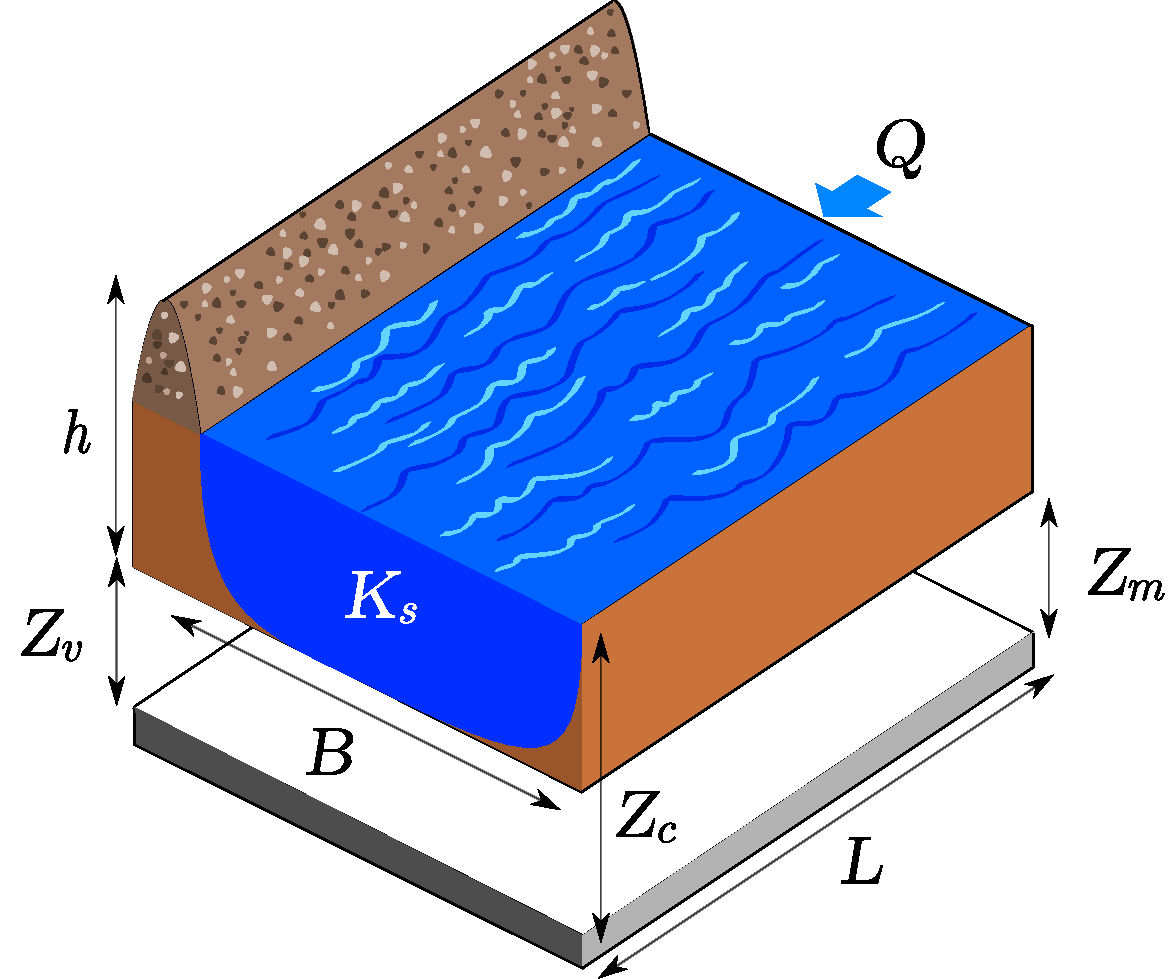
\includegraphics[width=9cm]{figures/river_section_large_adjusted} 
\end{center}
\caption{The flood example: simplified model of a river.}\label{fig:crues}
\end{figure}

\begin{table}[!ht]
  \begin{center}
   \begin{tabular}{lccc}
Input & Description & Unit & Probability distribution \\
   \hline
 $Q$ & Maximal annual flowrate & m$^3$/s & Gumbel ${\mathcal G}(scale = 558, mode = 1013)$ \\
 $K_s$ & Strickler coefficient & - & Normal ${\mathcal N}(30, 7.5)$  \\
 $Z_v$ & River downstream level & m & Uniform  ${\mathcal U}(49, 51)$ \\
 $Z_m$ & River upstream level  & m  & Uniform  ${\mathcal U}(54, 56)$\\
\hline
    \end{tabular}
    \caption{Input variables of the flood model and their probability distributions.}
    \label{tab:factors}
  \end{center}
\end{table}

The goal of this study is twofold:
\begin{itemize}
\item we want to estimate the mean river height $E(S)$, 
\item we want to perform the sensitivity analysis of the model, i.e. 
we want to rank the inputs $Q$, $K_s$, $Z_v$ and $Z_m$.
\end{itemize}

%%%%%%%%%%%%%%%%%%%%%%%%%%%%%%%%%%%%%%%%%%%%%%%%%

\section{Define the random vector}

We beging by importing the required modules.
\lstset{language=Python}
\begin{lstlisting}
from openturns.viewer import View
import openturns as ot
from math import sqrt
import pylab as pl
\end{lstlisting}


We first define the function through which we want to propagate the uncertainties with the 
\pyobj{def} operator.

\lstset{language=Python}
\begin{lstlisting}
def functionFlood(X) :
    Hd = 3.0
    Zb = 55.5
    L = 5.0e3
    B = 300.0
    Zd = Zb + Hd
    Q, Ks, Zv, Zm = X
    alpha = (Zm - Zv)/L
    H = (Q/(Ks*B*sqrt(alpha)))**(3.0/5.0)
    S = H + Zv
    return [S]
\end{lstlisting}

Then we convert this Python function into an OpenTURNS function with the 
\pyobj{PythonFunction} class. 

\lstset{language=Python}
\begin{lstlisting}
input_dimension = 4
g = ot.PythonFunction(input_dimension, 1, functionFlood)
\end{lstlisting}

Now we create the distributions for the input variables.
\begin{itemize}
\item There are several ways to set the parameters of the Gumbel distribution for the $Q$ variable. 
Here the parameters are defined with the scale and mode parameters, which corresponds to the 
\pyobj{GumbelAB} class.
\item The $Q$ and $K_s$ variables must remain positive (a negative value is not compatible with the 
physical model). 
For this reason, we must truncate the distribution with 
\pyobj{TruncatedDistribution}.
\end{itemize}

\begin{lstlisting}
myParam = ot.GumbelAB(1013., 558.)
Q = ot.ParametrizedDistribution(myParam)
otLOW = ot.TruncatedDistribution.LOWER
Q = ot.TruncatedDistribution(Q, 0, otLOW)
Ks = ot.Normal(30.0, 7.5)
Ks = ot.TruncatedDistribution(Ks, 0, otLOW)
Zv = ot.Uniform(49.0, 51.0)
Zm = ot.Uniform(54.0, 56.0)
\end{lstlisting}

We set the descriptions of the random variables: they are used for the graphics.
\begin{lstlisting}
Q.setDescription(["$Q (m^3/s)$"])
Ks.setDescription(["$Ks (m^{1/3})/s)$"])
Zv.setDescription(["Zv (m)"])
Zm.setDescription(["Zm (m)"])
\end{lstlisting}

The \pyobj{drawPDF} presents the probability distribution function of the variable. 
\begin{lstlisting}
Q.drawPDF()
\end{lstlisting}
The following session produces the figure \ref{fig-variableQ}.
When we 
closely look at the PDF of $Q$, we see a small increase of the density for $Q=0$, because of the 
truncation of the distribution.


\begin{figure}
\centering
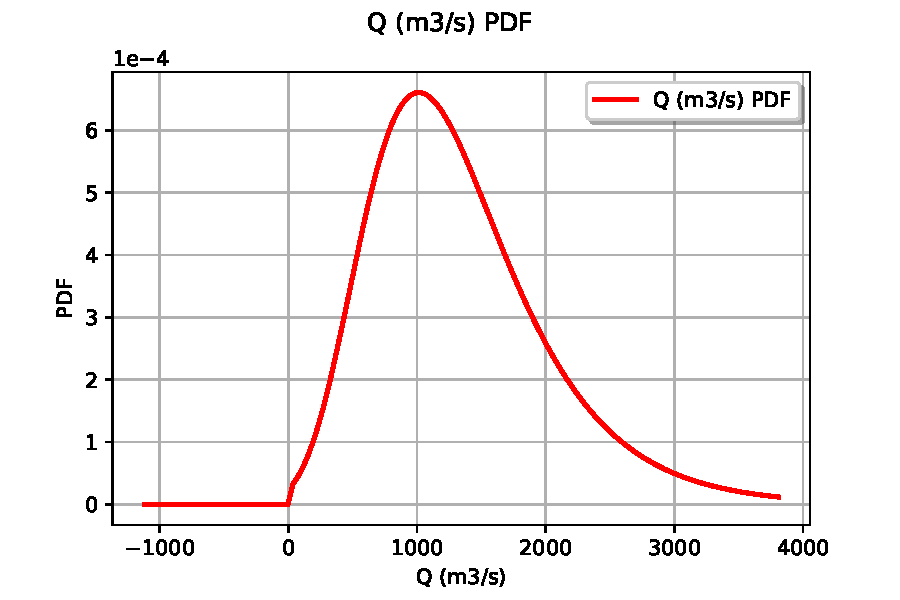
\includegraphics[width=0.8\textwidth]{figures/inputVariableQ.pdf}
\caption{The probability density function of the variable $Q$.}
\label{fig-variableQ}
\end{figure}

Then we create the input random vector \pyobj{inputvector}: by default, the copula is independent. 
Finally, we create the output vector \pyobj{S}.
\begin{lstlisting}
X = ot.ComposedDistribution([Q, Ks, Zv, Zm])
inputRV = ot.RandomVector(X)
S = ot.RandomVector(g, inputRV)
\end{lstlisting}

These steps are typical of probabilistic programming: we 
have defined the random variables involved in the problem 
without having generating a sample \emph{so far}.

%%%%%%%%%%%%%%%%%%%%%%%%%%%%%%%%%%%%%%%%%%%%%%%%%

\section{Estimating the mean with an incremental algorithm}

%%%%%%%%%%%%%%%%%%%%%%%%%%%%%%%%%%%%%%%%%%%%%%%%%

\subsection{Theory}

In this section, we the principles that are used in a new incremental 
algorithm in OpenTURNS 1.12 ; the goal of this algorithm is to estimate the mean of a random variable. 

Assume that the output $Y\in\mathbb{R}^{n_Y}$ is a random vector and that we want to estimate the 
mean $E(Y)$. 

The Monte Carlo algorithm  with the sample mean : 
$$
\overline{Y} = \frac{1}{n} \sum_{i=1}^n Y_i
$$
where $n$ is the sample size and $Y_i$ are i.i.d. realizations of the output. 

We use the fact that the sample mean is asymptotically gaussian :
$$
\overline{Y} \sim \mathcal{N}\left(E(Y),\frac{V(Y)}{n}\right).
$$
where $V(Y)$ is the variance of the output and $n$ is the sample size.

In general, most users set the sample size $n$ in advance and estimate the precision afterwards. 
Instead, suppose that if set the absolute precision and wish to determine the smallest sample 
size $n$ that achieves this precision. 
If we knew the variance $V(Y)$, we could set the value of $n$ 
so that the standard deviation $\sqrt{V(Y)}$ would be small enough. 
If instead we want to set the 
relative precision, we could consider the coefficient of variation $\frac{\sqrt{V(Y)}}{E(Y) 
\sqrt{n}}$ as a criterion (if $E(Y)\neq 0$). 
However, we obviously do not know the value of neither $E(Y)$ nor $V(Y)$. 

The purpose of the algorithm is to increase the 
sample size $n$ incrementally until a stopping criteria is met. 
At each iteration, we approximate the values of $E(Y)$ and $V(Y)$ by their 
empirical estimators. 

This algorithm works by updating a sample which size increases progressively until a stopping 
criteria is met. 
In order to get the best possible performance on distributed supercomputers and 
multi-core workstations, the size of the sample increases by block. 
For exemple, if the block size is equal to 100, then the sample size will be equal to 0, 100, 
200, etc... 
On each block, the evaluation of the outputs can be parallelized, which allows to improve the 
performance of the algorithm.

There are three mathematical stopping criteria available:
\begin{itemize} 
\item through an operator on the coefficient of variation $\frac{\sigma_i}{\mu_i}$ (a relative criterion)
\item through an operator on the standard deviation $\sigma_i$ (absolute criterion)
\item on the maximum standard deviation per component: $\sigma_i \leq \max_{i=1,...,n_Y} \sigma_i$ (absolute criterion)
\end{itemize} 

By default, the maximum coefficient of variation is used, i.e. the algorithm stops when: 
$$
\max_{i=1,...,n_Y} \frac{\sigma_i}{\mu_i} \leq max_{COV}.
$$
%%%%%%%%%%%%%%%%%%%%%%%%%%%%%%%%%%%%%%%%%%%%%%%%%

\subsection{Tutorial}

In this section, we present how to use the \pyobj{ExpectationSimulationAlgorithm} class 
in the tutorial flooding example. 
We set the maximum number of iterations with the \pyobj{setMaximum\-OuterSampling} so that 
we use at most 1000 iterations. 
In order to evaluate the function with blocks of size 10, we use the \pyobj{setBlockSize}. 
In this simulation, we use a relative stopping criteria and configure the 
maximum coefficient of variation to be equal to 0.001.
\begin{lstlisting}
algo = ot.ExpectationSimulationAlgorithm(S)
algo.setMaximumOuterSampling(1000)
algo.setBlockSize(10)
algo.setMaximumCoefficientOfVariation(0.001)
\end{lstlisting}
The computationnaly intensive part of the simulation is associated with the 
\pyobj{run} method. 
\begin{lstlisting}
algo.run()
\end{lstlisting}
Once the simulation is done, the \pyobj{getResult} method allows to 
access to the results.
\begin{lstlisting}
result = algo.getResult()
expectation = result.getExpectationEstimate()
print("Mean = %f " % expectation[0])
print("Number of calls to G = %d" % g.getCallsNumber())
\end{lstlisting}
The previous session prints the following output.
\begin{lstlisting}
Mean = 52.520729 
Number of calls to G = 500
Coef. of var.=0.000994
\end{lstlisting}
The estimate of the mean has a known asymptotical gaussian distribution, which can be retrieved 
with the \pyobj{getExpectation\-Distribution} method.
\begin{lstlisting}
expectationDistribution = result.getExpectationDistribution()
print(expectationDistribution)
View(expectationDistribution.drawPDF())
\end{lstlisting}
We emphasize that the output of the \pyobj{getExpectation\-Distribution} method is 
a \pyobj{Distribu\-tion} in the OpenTURNS sense: the whole information is available, 
not just a part of it, making the output as programmatically meaningful as possible. 
\begin{lstlisting}
expectationDistribution = result.getExpectationDistribution()
expectationDistribution.drawPDF()
\end{lstlisting}
The previous script produces the figure \ref{fig-variableMeanS}. 
The figure shows that we have an accurate estimate of the mean, 
up to approximately 2 significant digits. 

\begin{figure}
\centering
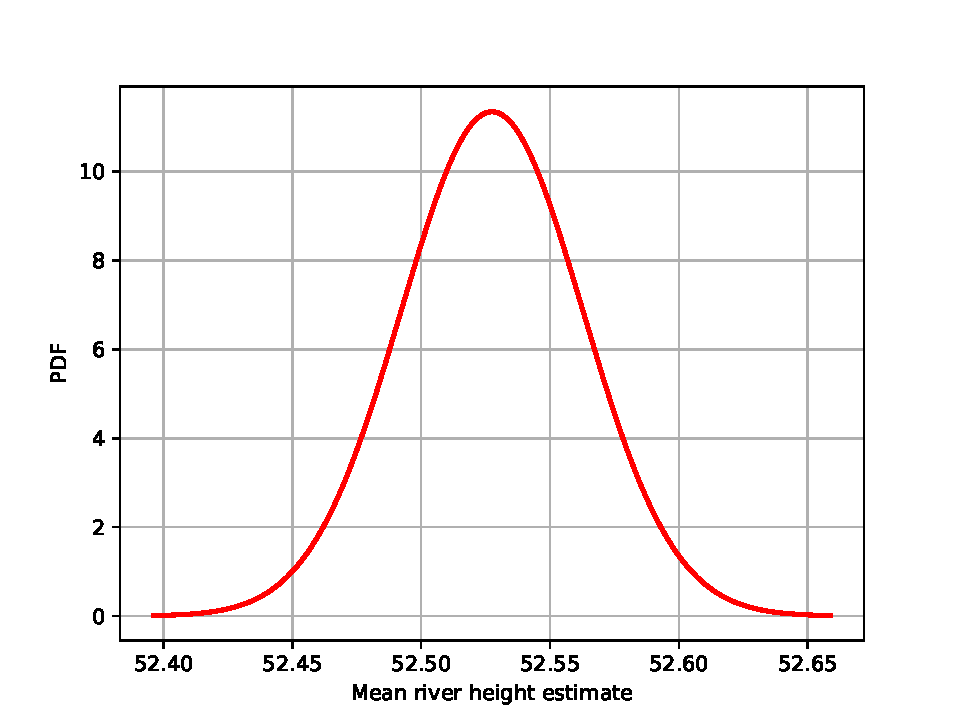
\includegraphics[width=0.8\textwidth]{figures/MeanSDistribution.pdf}
\caption{The probability density function of the estimate 
of the mean of the river height.}
\label{fig-variableMeanS}
\end{figure}

%%%%%%%%%%%%%%%%%%%%%%%%%%%%%%%%%%%%%%%%%%%%%%%%%

\section{Estimate sensitivity indices with an incremental algorithm}

\subsection{Theory}

In this section, we the principles that are used in a new incremental 
algorithm in OpenTURNS 1.12 which computes the Sobol' sensitivity 
indices. 

In \cite{Janon2014} the authors derive a new method to estimate the 
Sobol' sensitivity indices ; one of the advantages of the new 
estimator is that it is associated with an asymptotic distribution, 
which is derived thanks to the so called "delta"-method. 
Based on a suggestion by R.Lebrun, A. Dumas \cite{RapportSobol2018} 
used the same theoretical method in order to derive the 
asymptotic distribution of Sobol' sensitivity indices already available 
in OpenTURNS. 

\subsubsection{Overview}

Let us denote by $X\in\mathbb{R}^{n_X}$ a random vector. 
This algorithm works in the general case where the output $Y\in\mathbb{R}^{n_Y}$ is a random 
vector : in this case it operates on aggregated indices. 
In order to simplify the discussion, let us make the hypothesis that $n_Y=1$. 

The Sobol' first order sensitivity indices are defined by 
$$
S_i = \frac{V(E(Y|X_i))}{V(Y)}
$$
for $i=1,...,n_X$. The total order sensitivity indices are defined by :
$$
T_i = 1 - \frac{V\left(E\left(Y|X_{-i}\right)\right)}{V(Y)}
$$
where $-i$ is the set of indices which are different from $i$. 
In the remaining of this section, 
we focus on the first order sensitivity indice and let the reader consider [1] for the total 
order indices. 
Moreover, the derivation is the same for all input variables so that we omit the 
indice $i$ in order to simplify the notations. 

\subsubsection{Asymptotic distribution}

The algorithm is based on the fact that the estimatores of the 
first and total order Sobol' sensitivity indices 
asymptotically have the gaussian distribution. 
This gaussian distribution can be derived from the 
so called "delta"-method. 

Assume that the Sobol' estimator is 
$$
\overline{S} = \Psi\left(\overline{U}\right)
$$
where $\Psi$ is a multivariate function, $U$ is a multivariate sample and $\overline{U}$ is its 
sample mean. 
Each Sobol' estimator can be associated with a dedicated choice of function $\Psi$ 
and vector $U$. 

Let us denote by $\Phi_j^F$ (resp. $\Phi_j^T$) the cumulated distribution function of the 
gaussian distribution of the first (resp. total) order sensitivity indice of the j-th input 
variable.

Each available estimator in the library provides its own distribution, namely 
the Saltelli, Mauntz-Kucherenko, Jansen and Martinez estimators.

\subsubsection{Stopping criteria}
We set $\alpha\in[0,1]$ the level of the confidence interval and $\epsilon \in(0,1]$ the length 
of the confidence interval. 
The algorithms stops when, on all components, one of the two 
following conditions are satisfied :
\begin{itemize}
\item first and total order indices haved been estimated with enough precision or 
\item the first order indices are separable from the total order indices. 
\end{itemize}

The precision is said to be sufficient if the $1-2\alpha$ confidence interval is smaller than 
$\epsilon$ :
$$
(\Phi_j^F)^{-1}(1-\alpha) - (\Phi_j^F)^{-1}(\alpha) \leq \epsilon
$$
and 
$$
(\Phi_j^T)^{-1}(1-\alpha) - (\Phi_j^T)^{-1}(\alpha) \leq \epsilon
$$
for $j=1,...,n_X$.  
The first order indices are \emph{separable} from the total order indices if 
$$
\Phi_j^F(1-\alpha) \leq \Phi_j^T(\alpha)
$$
for $j=1,...,n_X$.  
This criteria allows to stop when the algorithm has detected an interaction 
between input variables with sufficient precision. 

%%%%%%%%%%%%%%%%%%%%%%%%%%%%%%%%%%%%%%%%%%%%%%%%%

\subsection{Tutorial}

In this section, we present how to use the \pyobj{SaltelliSensitivityAlgorithm} classe 
in the tutorial flooding example. 


We first set the parameters of the algoritms. 
We set the \pyobj{alpha} variable so that a 90\% confidence interval is used. 
In order to get confidence intervals which are not greater than 0.2, we set 
the variable \pyobj{epsilon} variable accordingly. 
The block size corresponds to the size of the Sobol' design of experiment generated 
at each iteration. 
Finally, the \pyobj{batchsize} variable contains the number of points evaluated simultaneously 
by the model. 
\begin{lstlisting}
alpha = 0.05 # 90% confidence interval
epsilon = 0.2 # Confidence interval length
blocksize = 50 # Size of Sobol experiment at each iteration
batchsize = 16 # Number of points evaluated simultaneously
\end{lstlisting}

Then we create the algorithm and configure the algorithm so that it 
uses the previous variables. 
Moreover, we configure the algorithm so that at most 100 iterations are used. 
\begin{lstlisting}
estimator = ot.SaltelliSensitivityAlgorithm()
estimator.setUseAsymptoticDistribution(True)
algo = ot.SobolSimulationAlgorithm(X, g, estimator)
algo.setMaximumOuterSampling(100) # number of iterations
algo.setBlockSize(blocksize) 
algo.setBatchSize(batchsize) 
algo.setIndexQuantileLevel(alpha) # alpha
algo.setIndexQuantileEpsilon(epsilon) # epsilon
algo.run()
\end{lstlisting}

Once that the algorithm has run, the results can be retrieved and estimates 
of first and total order indices can be printed. 
\begin{lstlisting}
result = algo.getResult()
fo = result.getFirstOrderIndicesEstimate()
to = result.getTotalOrderIndicesEstimate()
print("First order = %s" % (str(fo)))
print("Total order = %s" % (str(to)))
\end{lstlisting}

The previous script produces the following output.
\begin{lstlisting}
First order = [0.529059,0.205321,0.381215,0.0316592]
Total order = [0.481355,0.130565,0.362292,0.011206]
\end{lstlisting}

We can obtain the asymptotic distribution of the first and total 
order indices. 
For example, the following script extracts the first component of the 
asymptotic distribution of the first order indice (which corresponds to the variable 
$Q$) and plots it.
\begin{lstlisting}
dist_fo = result.getFirstOrderIndicesDistribution()
dist_fo_i = dist_fo.getMarginal(0)
graph = dist_fo_i.drawPDF()
graph.setTitle("S0")
graph.setXTitle("S0")
\end{lstlisting}
The previous script produces the figure \ref{fig:asymptQ}.

\begin{figure}[!ht]
\begin{center}
    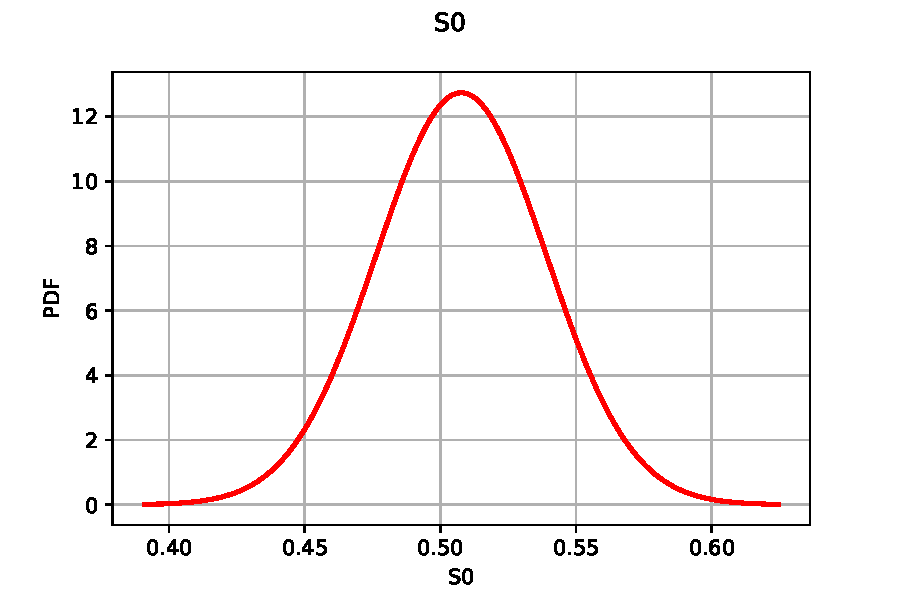
\includegraphics[width=9cm]{figures/S0-distribution} 
\end{center}
\caption{Asymptotic distribution of the first order Sobol' indices 
for the $Q$ variable.}
\label{fig:asymptQ}
\end{figure}

In order to get a more compact view of the first and total order indices 
along with their confidence intervals, we often represent the 90\% confidence 
intervals with a vertical bar. 
The figure \ref{fig:sobolindices} presents the Sobol' indices with 
asymptotic confidence intervals. 
We observe that the the confidence intervals are relatively small, 
as expected. 

\begin{figure}[!ht]
\begin{center}
    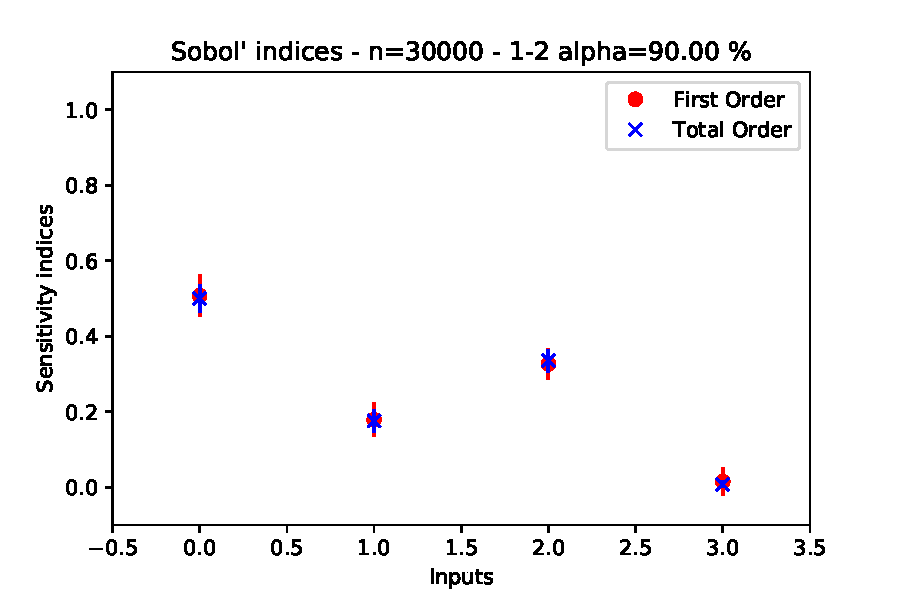
\includegraphics[width=9cm]{figures/crue-Sobol-indices} 
\end{center}
\caption{Sobol' indices with asymptotic confidence intervals.}
\label{fig:sobolindices}
\end{figure}

%
% BibTeX users please use
\bibliographystyle{plain}
\bibliography{otgui}


%%%%%%%%%%%%%%%%%%%%%%%%%%%%%%%%%%%%%%%%%%%%%%%%%%%%%%%%%%%%%%%%%%%%%%

\end{document}
